\chapter{Working context}\label{chap:organisation}

\section{Planning}
\subsection{Discovering the code}
At the first work week, I dug into the Parameter-framework's code. I had no
documentation at all, just the code on \gls{GitHub}. The absence of help was done on
purpose: the team needed an external point of view on the source code. I had
to understand the powerful concepts of the Parameter-framework just by reading
the code. Since I struggled a bit with the concepts, I decided to write some
newcomer tutorials which content are described at section \ref{sec:tutorials}.
I started to submit code quite early (the second week), with \gls{pullrequests} on \gls{GitHub}.

\subsection{Joining forces with the scrum team}
After three weeks, I requested to join a \gls{scrum} team so that I could experience
Intel's way of working with \gls{scrum}!
The rest of my internship I was considered as an \emph{agile developer}, completely member of the team.
In section \ref{sec:agile}, I describe a bit more the agile methodology.

\subsection{Gantt chart}
Since I worked as an agile developer, I had no long term goal to reach. This
Gantt chart is more like a trace of my different activities than a real planning
diagram.

%\end{figureGraphics}

% Improving build process
% Xml checker
% Multi-variant support
% Fixed point enhancements
% Multi modem support

% Newcomer documentation
% Intellectual property
% Alsa plugin refactor
% Filesystem plugin update
% Core update
% Alsa plugin update

% Internship report

\begin{figureGraphics}{Gantt chart}{fig:gantt}
    \hspace*{-2cm}
\begin{ganttchart}[
        x unit=0.5cm,
        y unit title=.6cm,
        y unit chart=.6cm,
        hgrid=true,
        vgrid={*1{red,  dotted}},
        canvas/.style={fill=base2},
        bar/.style={fill=orange},
        title/.style={fill=base2},
        group/.style={fill=blue, shape=ganttgroup},
        bar height = 0.4,
    ]{1}{24}
    \gantttitlelist{1, ..., 24}{1} \\
    \ganttgroup{Enchancements}{4}{20} \\
    \ganttbar{Arrival, installation}{1}{1} \\
    \ganttbar{Improving build process}{4}{11} \\
    \ganttbar{Multi-variant support}{5}{6} \\
    \ganttbar{Fixed point enhancements}{9}{11}\\
    \ganttbar{Multi modem support}{17}{20}\\
    \ganttgroup{Open-sourcing}{1}{20} \\
    \ganttbar{Newcomer documentation}{1}{4}\\
    \ganttbar{Intellectual property}{12}{13}\\
    \ganttbar{Alsa plugin refactor}{12}{14}\\
    \ganttbar{Filesystem plugin update}{14}{15}\\
    \ganttbar{Core update}{15}{18}\\
    \ganttbar{Alsa plugin update}{17}{20}\\
    \ganttgroup{University}{21}{24} \\
    \ganttbar{Internship report}{21}{24}
\end{ganttchart}
\end{figureGraphics}

Every task has a dedicated section in this document to describe what have been done.
This can be found in chapter \ref{chap:contributions}.


\section{Agile methodology}\label{sec:agile}

In the team I was working, we were organized around Agile software
development. This way of working promotes incremental results and adaptive planning.
There are several implementations of Agile methods. In our team we were using \gls{scrum}.

In order to understand how I worked during my internship, some key concepts of \gls{scrum} must be described.

\subsection{Key concepts}

\subsubsection{Story}\label{sec:story}
A story is a \emph{business-oriented}, short description of a client's need.
Most of the times, it is divided into several tasks so that the developers
can take small steps to complete the story. A story is usually printed or
written on sticky note. Those notes are grouped on a story board (see figure
\ref{fig:storyboard}). When a developer starts to work on a new Story, he takes
the sticky note and moves it on the board.

\begin{figureGraphics}{A story board}{fig:storyboard}
    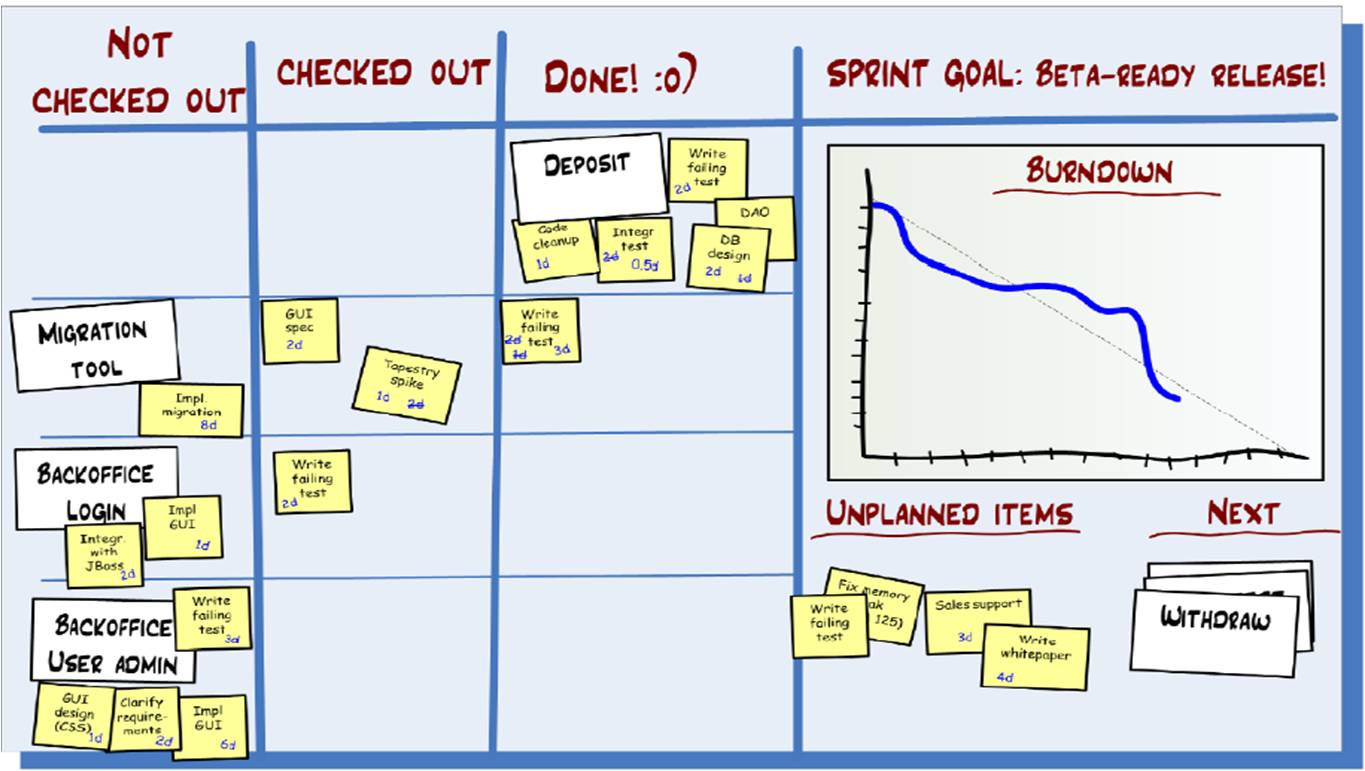
\includegraphics[width=\textwidth]{./src/img/taskboard.jpg}
\end{figureGraphics}


\subsubsection{Sprints}\label{sec:sprint}
Sprints are short development cycles, usually from one to four weeks. We were
delivering results every three weeks. During each sprint, a team creates a
shippable product, no matter how basic that product is. A sprint is composed of
a set of stories which should be completed at it's end.

The interesting part of working in sprints is the idea of "making a fresh start" every three weeks. This
was quite motivating to me!


\subsection{Team}
Our team is composed of six members(me included); all software engineers with various
skills. Some are more software design oriented while others are more hardware
specialists.

Within the team, some members have a particular role:
\begin{description}
    \item[The Product owner]
        defines what the team is doing during a Sprint (see \ref{sec:sprint}).
        He determines the priority of each story (see \ref{sec:story}) the
        team is working on. His input usually comes from clients. He is the
        business-oriented person in the team. His decisions have an impact on
        the results a \gls{scrum} team delivers. Usually, he is not
        a part of the \gls{scrum} team.
    \item[The scrum master]
        ensures that every team member is correctly focused on his story. He
        is keeping track of the progress of each member and should alert the
        Product owner when some impediments appear (bad time estimation of a
        story, blocking facts due to hardware, ...).
\end{description}

Note that in our team, the Product owner and the \gls{scrum} master were also contributing to the team as software engineers.

\subsection{Events}
In \gls{scrum}, there are several events occurring during a sprint.
These are essential to the \gls{scrum} methodology.

\subsubsection{Daily scrum}\label{sec:daily}
Every day, at 11:30 we were holding the daily \gls{scrum} meeting, also called "stand-up".
During that time, each member of the team answers quickly the three following questions:

\begin{description}
    \item[What have I done since yesterday ?]
    \item[What am I planning for today ?]
    \item[Any issues encountered ?]
\end{description}

This meeting is very useful, it helps tackle early problems and can assist the \gls{scrum} master to detect delays in delivering.
Note that this should not take longer than 15 minutes.


\subsubsection{Planning poker}
During planning poker sessions, we have to estimate how much time each story takes. In order to do a correct estimate,
the product owner is explaining what the exact requirements are. After that, each member of the team should guess
how much "story points" (which can sometimes be approximated to a day of work) the story should take to be done.
This is done in the form of a vote, with poker session cards.

\begin{figureGraphics}{Planning poker cards}{fig:poker}
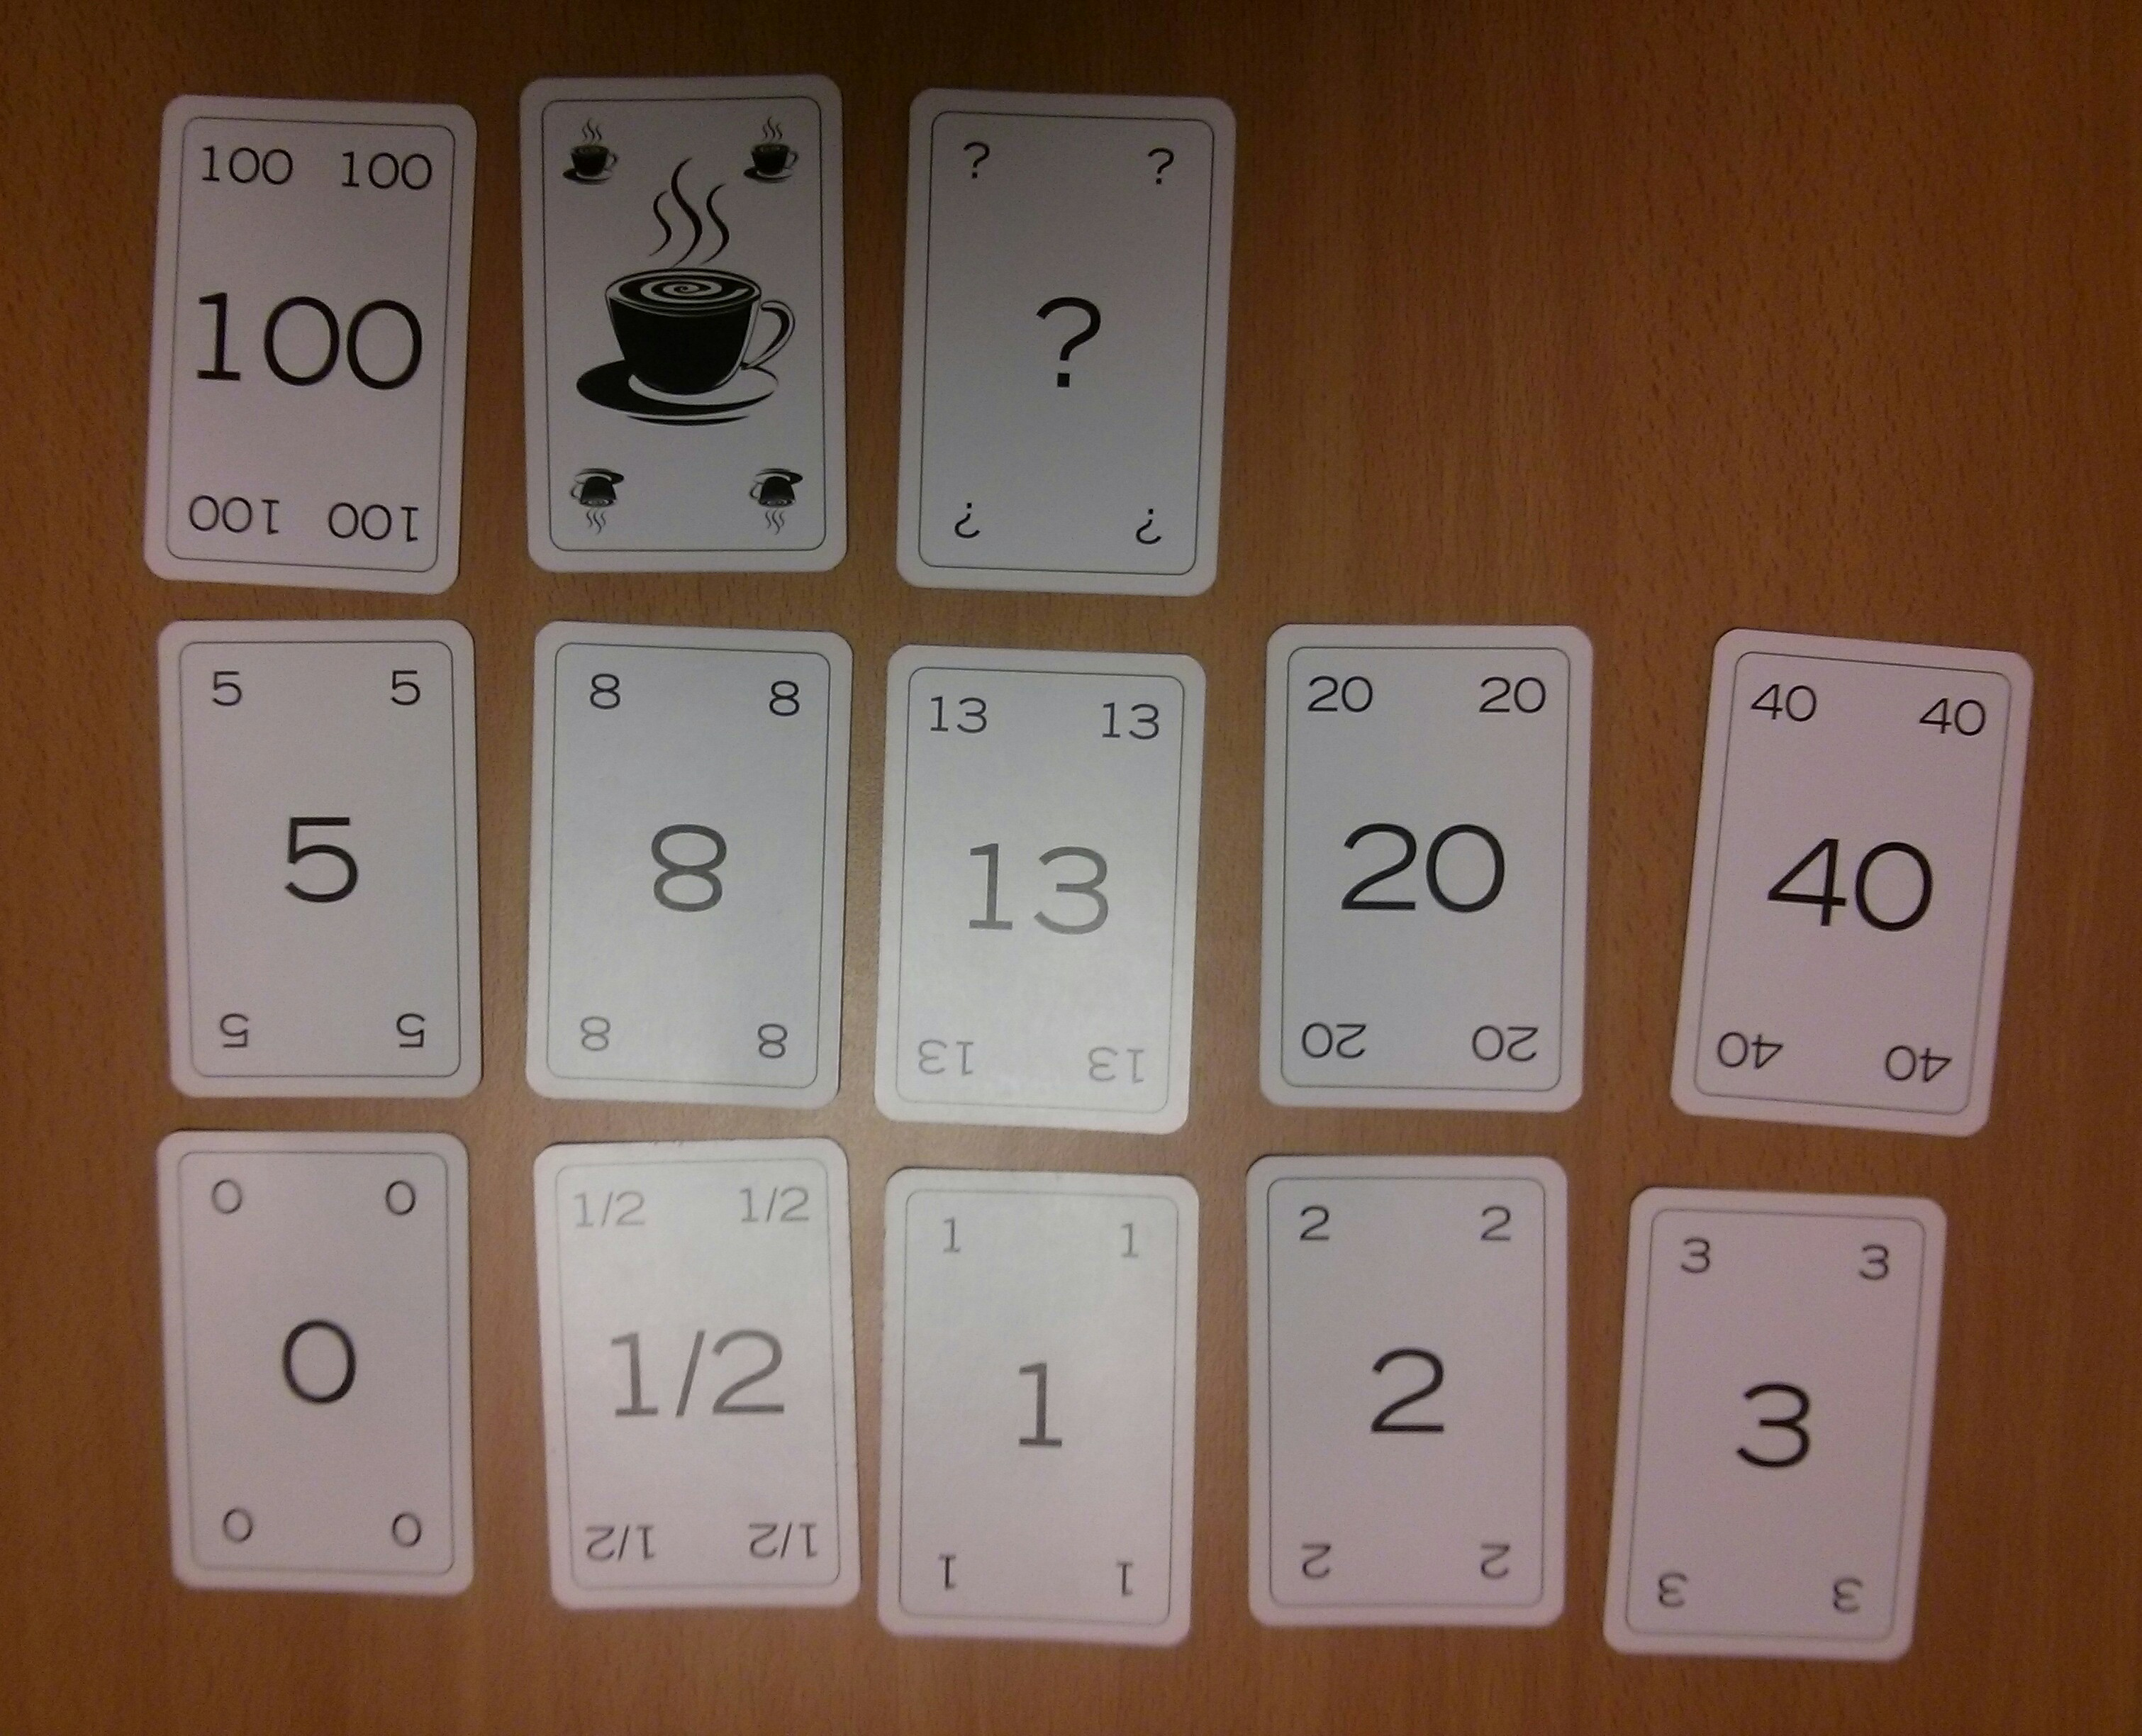
\includegraphics[width=\textwidth]{./src/img/poker.jpg}
\end{figureGraphics}

After arriving at a team consensus, the story is considered \emph{planned}. This
is very useful so that the Product owner can group multiple stories which have
to be done in a sprint.


\subsubsection{Demos}
At the end of each sprint, the team has to demonstrate their achievements. This
is a very important meeting with people external to the team, usually clients.
Since our development team haves no "client" in standard sense, the audience of our demos are
the integration team and the architect team.
Only the work which was \emph{done} during the last sprint is showed off during that presentation.

This presentation is important to show the contributions that the team has made.
I participated in every Demo since I was fully member of the \gls{scrum} team.

\subsubsection{Retrospectives}
After the Demo, the team has a look back at how the last sprint happened. This short meeting is made
to find out what the team did wrong last sprint, but also to highlight what the team did right!
It is frequent to see little psychological games during the retrospective, which makes all members more
eager to participate.
